\documentclass[a4paper,11pt]{book}

% Paketi za nas jezik (optimalni)
\usepackage{cmsrb}
\usepackage[OT2,T1]{fontenc}
\usepackage[serbian]{babel}

\usepackage{graphicx}
\usepackage{lmodern}
\usepackage{hyperref}


\makeatletter
\newenvironment{chapquote}[2][2em]
  {\setlength{\@tempdima}{#1}%
   \def\chapquote@author{#2}%
   \parshape 1 \@tempdima \dimexpr\textwidth-2\@tempdima\relax%
   \itshape}
  {\par\normalfont\hfill--\ \chapquote@author\hspace*{\@tempdima}\par\bigskip}
\makeatother

\title{\Huge \textbf{Modelovanje autonomnog sistema za kompaktan uzgoj biljaka} \\ \huge Modelovanje i simulacije}
\author{\textsc{Aleksandar Stojanović RN97-2018}}


\begin{document}

\maketitle
\tableofcontents

%\mainmatter
\chapter*{Uvod}

\section*{Svrha rada}
Ovaj rad je stvoren sa ciljem da opiše jednostavno i pristupačno rešenje za proizvodnju hrane u veštačkim uslovima.

\noindent U ovom radu prezentovaću svoj pristup dizajniranja ovakvog sistema. Detaljno cu analizirati principe rada individualnih podsistema koji sačinjavaju ovu jedinicu i simulirati njihov rad.

\section*{Uzgoj u zastvorenom prostoru}
Ovakav vid proizvodnje sa urbanizacijom postaje sve popularniji. Kako gradovi postaju sve veći, potreba za organskom hranom raste te se ljudi okreću alternativnim metodama uzgoja.

Kada je reč o zatvorenim prostorima, u glavnom se misli na kontrolisano okruženje koje ima za cilj da olakša razvoj biljke pa kasnije i samih plodova. Ovo se postiže adekvatnim planiranjem što podrazumeva razmatranje, ispunjavanjem svih uslova neophodnih za rast. 

\section*{Tradicionalan ili zatvoren uzgoj}
Dok nam tradicionalan pristup uzgoju olakšava logistiku i nudi dosta pogodnije mogućnosti za ekspanzije, zatvoren pristup pruža kompletno kontrolu nad samim okruženjem. Pored toga biljka je kopletno izolovana od negativnih spoljašnjih faktora kao što su:

\begin{itemize}
  \item paraziti,
  \item naglih oscilacija temperature,
  \item prevelike količine padavina.
\end{itemize}

\noindent Sama činjenica da je biljka u izolovanom okruženju nam omogućava da bliže pratimo njen razvoj. Ovo posebno dolazi do izražaja kod otkrivanja problema u ranim fazama.

\chapter{Priprema}

%\begin{chapquote}{Author's name, \textit{Source of this quote}}
%``This is a quote and I don't know who said this.''
%\end{chapquote}

\section{Definisanje problema}
Dakle, naš cilj je izrada autonomne jedinice koja radi bez čovekovog prisustva. Kako bismo to postigli moramo se osloniti na nekakvu upravljačku jedinicu koja ce biti zadužena za kontrolu celokupnog sistema uz oslonac na senzore. 

Glavna prepreka je limitirana količina prostora koja nam je na raspolaganju. Kada je reč o uzgoju u zatvorenim prostorima podrazumeva se da nam je sam prostor jako važan resurs i potrebno je iskoristiti ga što efikasnije. Tek kada je prostor pravilno iskorišćen možemo započeti optimizaciju ostlaih delova sistema.

Da bismo prostor koristili efektivno bitno je da unapred definišemo neke od funkcionalnosti našeg sistema: 

\hrulefill

1. Merenje i regulacija temperature,

2. Merenje vlažnosti zemlje i ambijenta,

3. Regulacija svetlosnog ciklusa,

4. Regulacija brzine ventilatora,

5. Zalivanje biljke,

6. Logovanje 

\hrulefill

\noindent Imajuci ove funkcije na umu mozemo odrediti grub plan projekta. U sledećoj tački ćemo da detaljo definisati svaku od ovih funkcija i opisati hardver koji ćemo koristiti za izradu.

\section{Plana izrade projekta}

Sistem će biti smešten u kabinet dimenzija 35x35x60 koji je izradjen od metala. Ova veličina ce podržati biljku srednjih veličina. Neophodno je da unutrašnjost kabineta bude obložena reflektivnim materijalom koji će dobrineti da biljka iskoristi pun potencijal svetla.

\noindent \\ Budući da ovakav sistem zahteva kontinualan rad sto podrazumeva dugoročno opterećenje, Adruino Uno\footnote{Arduino Uno je open-source rešenje u vidu kontrolera za IoT projekte koji pruža mnoštvo mogućnosti. Vise na: https://www.arduino.cc/en/Guide/Introduction} je idealno rešenje jer nudmi stabilnost pod dugoročnim radom i jednostavnu integraciju senzora. 

Pored stabilnosti ako pogledamo njegov dijagram(slika x.x) možemo uočiti da imamo izlaze od 3.3V i 5V sto je idealno za napajanje senzora i releja.

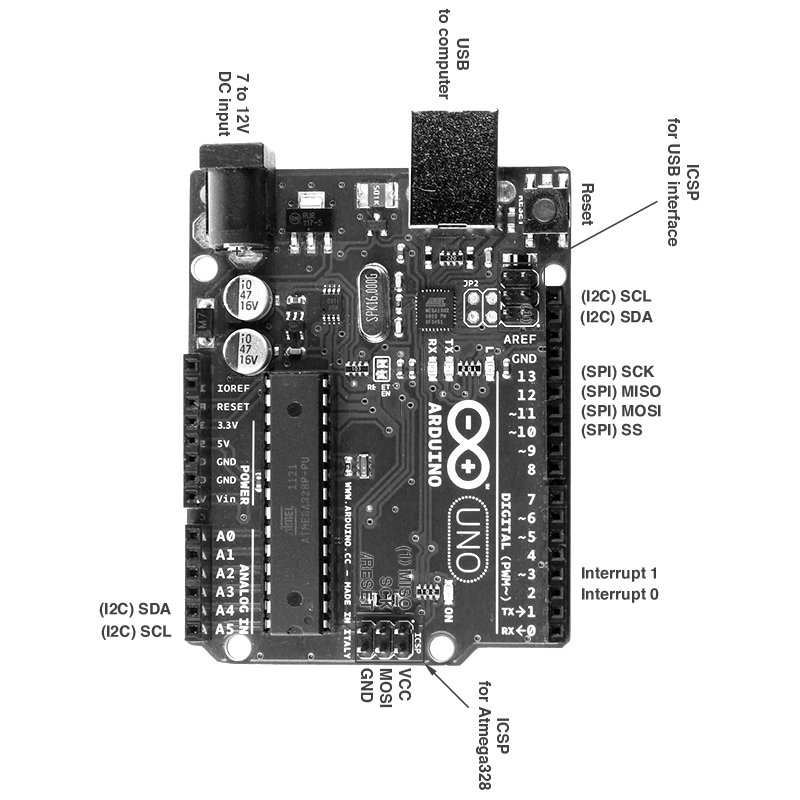
\includegraphics[width=\textwidth]{uno_pinout.png}

Kao monitor za feedback sistema koristicemo mali I2C\footnote{I2C protokol služi za serijsku komunikaciju sa mikrokontrolerima. Vise na: https://i2c.info/} OLED ekran velicine 0.11 inča kao dugoročno rešenje dok će serijski port biti primarno korišćen u početnim fazama izrade.

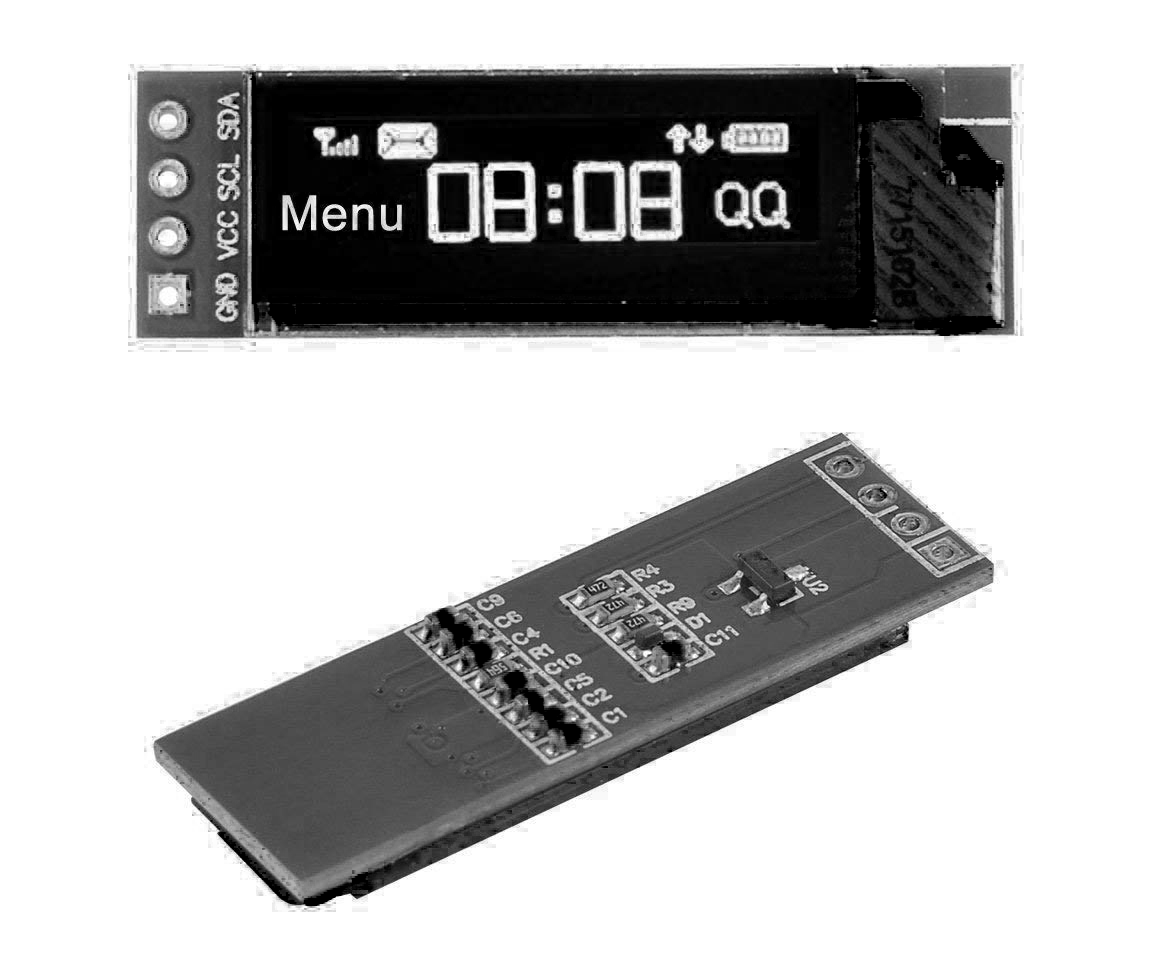
\includegraphics[width=\textwidth]{oled.png}

\subsection{Merenje temperature i regulacija}
Merenje temperature je krucijalan korak jer je to jedan od glavnih faktora okruženja. Različite biljke zahtevaju različite uslove poput povećane vlage, stoga neophodno je koristiti adekvatan hardver za nase uslove.\\ 

\noindent DS18B20\footnote{Digitalni senzor toplote koji nudi 9-bit do 12-bit vrednosti toplote izražene u celizijusu. Vise na: https://datasheets.maximintegrated.com/en/ds/DS18B20.pdf} je senzor po izboru iz razloga što je fabrički izolovan, ima dosta širi opseg vrednosti od očekivanog unutar sistema i napaja se sa 3.3V ili 5.5V.

Regulaciju rešavamo korišćenjem ulaznih i izlaznih ventilatora.

\subsection{Merenje vlažnosti zemlje i ambijenta}
Praćenjem vlažnosti zemlje nam omogućava da automatizovano zalivamo biljku u zavisnosti od njenih potreba. Za razliku od fiksnih ciklusa zalivanja kod kojih može doći do preteranog navodnjavanja ovde se mehanizam za navodnjavanje aktivira samo kada je to potrebno.

Za vlagu ambijenta koristimo HR202 senzor vlage u vazduhu, a za zemljiste koristimo kapacitivni senzor LDTR-WG0236.

\subsection{Regulacija svetlosnog ciklusa}
Različite biljke zahtevaju specifične svetlosne cikluse. Stoga, moramo konfigurisati naš kontroler po parametrima biljke kako bismo joj pružili optimalne uslove. Interval osvetljenja je konfigurisan softverski i zavisno od istog kontroler utiče na relej. 

Što se izbora tehnologije svetla tiče u opticaju imamo sledece:

\hrulefill
\begin{itemize}
  \item LED - Light emmiting diode
  \item HID - High-intensitz discharge
  \item Flourescent(CFL)
\end{itemize}
\hrulefill

\begin{table}[ht]
  \caption{Karakteristike različitih tehnologija}
  \begin{tabular}{|c|c|c|c|}
  \hline
   & CFL & HID & LED \\ \hline
  Inicijalna cena & Nisko & Srednje & Nisko/skupo \\ \hline
  Potrošnja & Nisko & Srednje/Visoko & Nisko \\ \hline
  Efikasnost & Osrednje & Dobro & Dobro/Odlično \\ \hline
  Udaljenost & Mala & Srednja & Srednja/Velika \\ \hline
  \end{tabular}
\end{table}

U našem slučaju, koristi se LED svetlo(150W - efektivno oko 90W) sa ugradjenim hladnjakom. Ova tehnologija je najbolja opcija za nas jer imamo dovoljno prostora a pored toga je jako isplativa.

\subsection{Regulacija rada ventilatora}
Ventilatori nam koriste za razmenu vazduha sa okolinom. Sa druge strane, kako utičemo na njihovu brzinu jedinica ce se brže odnosno sporije hladiti.

Da bismo pronašli odgovarajuću veličinu ventilatora za sistem moramo odrediti samo prostor sa kojim radimo:

\[ 35cm * 35cm * 60cm =  73500cm^3 = 2.595628ft^3\]

Iz ovoga vidimo da su nam dovoljno obicni 12V ventilatori. Budući da se na izlaz kači filter vazduha koji u sebi sadrži dva 60mm ventilatora koji po specifikaciji pomeraju 38.35cfm a nasa jedinica ima samo ~2.5, na ulaz možemo staviti jedan ventilator od 120mm koji cemo uključivati u slucaju da nam temperatura predje dozvoljenu. Ovo radimo sa ciljem da unutar jedinice stvorimo negativni pritisak (izbacuje se vise nego sto ulazi) kako bi obezbedili da nam vazduh izlazi samo na predvidjenom mestu.

\noindent Prebacivanjem izduva sa 9V na 12V i ukljucivanjem usisa na 9V sa kratkoročnim pauzama vrši se brža razmena toplote dok se temperature ne vrati na dozvoljeni nivo. 

\subsection{Zalivanje biljke}
Zalivanje biljke je jedan od elementarnih zahteva koje moramo ispuniti. Za ovo se koristi pumpa za vodu od 12V koja je potopljena u kanistar sa vodom. Pumpa se aktivira putem releja kada senzor vlage u zemlji detektuje niske količine vlage.

\noindent Od velikog značaja je ravnomerna distribucija vode unutar saksije kako bi senzor stvarao sto realniju sliku o stanju unutar iste.

\subsection{Logovanje}
Logovanje nam omogućava detaljnu analizu procesa i samog rada naše mašine ako se korektno implementira. Znatno olakšava otkrivanje greške ili kvara, pomaže u rešavanju i služi kao output sistema.

Generičan modul za sd kartice se koristi ovde koji ima sledeci pinout:

\hrulefill
\begin{itemize}
  \item VCC - 3.3V
  \item VCC - 5V
  \item MOSI
  \item CLK 
  \item MISO
  \item GND - ground
\end{itemize}
\hrulefill

Ovo ga čini idealnim za naše uslove. Na kartici će se beleziti svaki input koji sistem primi zajedno sa akcijom koja je izvrsena kroz vreme. Pored toga na kartici cemo cuvati parametre za biljku koja se trenutno uzgaja.

\section{Tehnički detalji}

Slika sistema

\chapter{Izgradnja modela}

Kada smo definisali hardver sistema možemo započeti izradu modela. U ovoj glavi posvetićemo se parametrima i njihovoj korelaciji unutar sistema.

\section{Konceptualizacija modela}

Kako bismo stvorili koncept modela moramo se vratiti na funkcije našeg sistema. Analizom funkcija i konkretnog hardvera pronalazimo matematički model koji predstavlja temelj naše simulacije.\\

\noindent Kroz sledeću tačku cemo se se baviti prikupljanjem podataka vezanih za nas sistem.

\section{Kolekcija podataka}



\section{Prevodjenje modela}

\section{Verifikacija}

\section{Validacija}

\chapter{Izvršavanje simulacije}

\section{Dizajn eksperimenta}

\section{Izvršavanje i analiza}

\section{Dodatna izvršavanja}

\chapter{Implementacija}

\section{Dokumentacija i izveštaj}

\section{Implementacija}

\end{document}

%\section*{Acknowledgements}
%\begin{itemize}
%\item A special word of thanks goes to Professor Don Knuth\footnote{\url{http://www-cs-faculty.stanford.edu/~uno/}} (for \TeX{}) and Leslie Lamport\footnote{\url{http://www.lamport.org/}} (for \LaTeX{}).
%\item I'll also like to thank Gummi\footnote{\url{http://gummi.midnightcoding.org/}} developers and LaTeXila\footnote{\url{http://projects.gnome.org/latexila/}} development team for their awesome \LaTeX{} editors.
%\item I'm deeply indebted my parents, colleagues and friends for their support and encouragement.
%\end{itemize}

%%%%%%%%%%%%%%%%%%%%%%%%%%%%%%%%%%%%%%%%%%%%%%%%%%%%%%%
% Sample table                                        %
% Source: www1.maths.leeds.ac.uk/latex/TableHelp1.pdf %
%%%%%%%%%%%%%%%%%%%%%%%%%%%%%%%%%%%%%%%%%%%%%%%%%%%%%%%
%\begin{table}[ht]
 % \caption{Sample table} % title of Table
  %\centering % used for centering table
  %\begin{tabular}{c c c c}
  % centered columns (4 columns)
  %\hline\hline %inserts double horizontal lines
  %S. No. & Column\#1 & Column\#2 & Column\#3 \\ [0.5ex]
  % inserts table
  %heading
  %\hline % inserts single horizontal line
  %1 & 50 & 837 & 970 \\
  %2 & 47 & 877 & 230 \\
  %3 & 31 & 25 & 415 \\
  % & 35 & 144 & 2356 \\
  %5 & 45 & 300 & 556 \\ [1ex] % [1ex] adds vertical space
  %\hline %inserts single line
  %\end{tabular}
  %\label{table:nonlin} % is used to refer this table in the text
  %\end{table}